\subsection{Grundlagen}
    \begin{definition}{{Matrix, Element, Zeilen, Spalten und Typ}}\\
        Eine \textit{Matrix} ist (simpel gesagt) ein Vektor mit mehreren Spalten 
        und wird mit Grossbuchstaben bezeichnet.
        Ein \textit{Element} $a_ij$ ist ein Wert aus dieser Matrix,
        auf den über die Zeile und Spalte zugegriffen wird (\textbf{Z}eile \textbf{z}uerst,
        \textbf{Sp}alte \textbf{Sp}äter).
        Der \textit einer Matrix ergibt sich aus der Anzahl ihren Zeilen und Spalten.
        Matrizen mit $m$-Zeilen und $n$-Spalten werden $m\times n$-Matrizen genannt.
    \end{definition}

    \begin{definition}{Nullmatrix}
        Eine Matrix, deren Elemente alle gleich $0$ sind, heisst \textit{Nullmatrix} und wird mit $0$ bezeichnet.
    \end{definition}

    \begin{definition}{Spaltenmatrix}
        \begin{wrapfigure}{hr!}{0.2\textwidth}
            \vspace{-20pt}
            \begin{equation*}
                \vec{a}=\begin{pmatrix}
                    a_1\\a_2\\\vdots\\a_n
                \end{pmatrix}
            \end{equation*}
        \end{wrapfigure}
        Besteht eine Matrix nur aus einer Spalte, so heisst diese \textit{Spaltenmatrix}.
        Spaltenmatrix können als Vektoren aufgefasst werden und können mit einem kleinen Buchstaben 
        sowie einem Pfeil darüber notiert werden ($\vec{a}$). 
    \end{definition}

    \begin{formula}{Addition und Subtraktion von Matrizen}\\
        Zwei Matrizen des gleichen Typs können addiert und subtrahiert werden.
        Diese Operationen werden Elementweise durchgeführt.
        \begin{center}
            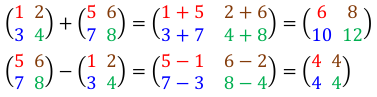
\includegraphics[width=0.5\linewidth]{mat-add-sub.png}
        \end{center}
    \end{formula}

    \begin{formula}{Skalare Multiplikation}
        Matrizen können mit einer $\lambda$ Zahl skaliert werden. Jedes Element wird dabei mit $\lambda$ multipliziert.
        \begin{center}
            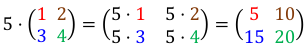
\includegraphics[width=0.5\linewidth]{mat-mul.png}
        \end{center}
    \end{formula}

    \begin{theorem}{Rechenregeln für die Addition und skalare Multiplikation von Matrizen}\\
        \begin{itemize}
            \item Kommutativ-Gesetz: $A+B=B+A$
            \item Assoziativ-Gesetz: $A+(B+C)=(A+B)+C$
            \item Distributiv-Gesetz:\\ 
                $\lambda\cdot(A+B)=\lambda\cdot A+\lambda\cdot B$
                sowie $(\lambda + \mu)\cdot A=\lambda\cdot A+\mu\cdot A$
        \end{itemize}    
    \end{theorem}

    \begin{definition}{Transponieren}
        \begin{wrapfigure}{r}{0.4\textwidth}
            \vspace{-13pt}
            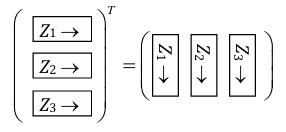
\includegraphics[width=0.9\linewidth]{mat-transpos.png}
        \end{wrapfigure}
        Die \textit{Transponierte} einer $m\times n$-Matrix ist eine $n\times m$-Matrix. 
        Diese wird erhalten, indem die Zeilen zu Spalten und die Spalten zu Zeilen gemacht werden.
    \end{definition}

    \begin{theorem}{Transposition Regeln}
        \begin{equation*}
            {(A\cdot B)}^T = B^T\cdot A^T
        \end{equation*}
    \end{theorem}

    \begin{definition}{Multiplikation von Matrizen}
        Die Multiplikation von Matrizen ist \textbf{nicht} elementweise definiert!
        Dammit zwei Matrizen $A$ und $B$ multipliziert werden können,
        muss die \textbf{Anzahl Spalen von $A$ gleich der Anzahl Zeilen von $B$}.
        Die Resultierende Matrix hat gleich viele Zeilen wie $A$ und Spalten wie $B$. 
        \begin{highlight}{<!>}
            Die Matrizenmultiplikation ist \textbf{nicht Kommutativ}!
        \end{highlight}
        \begin{center}
            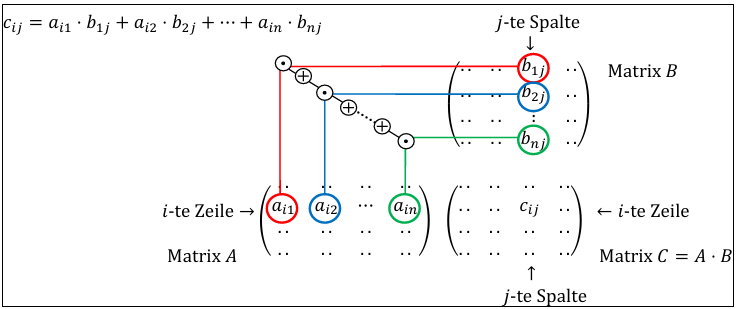
\includegraphics[width=0.8\linewidth]{mat-mat-mul.png}
        \end{center}
    \end{definition}
    
    \begin{theorem}{Rechenregeln für die Multiplikation von Matrizen}
        \begin{itemize}
            \item Assoziativ-Gesetz: $A\cdot(B\cdot C)=(A\cdot B)\cdot C$
            \item Distributiv-Gesetz: \\
                $A\cdot(B+C)=A\cdot B+A\cdot C$ und $(A+B)\cdot C=A\cdot C+B\cdot C$
            \item Skalar-Koeffizient: $(\lambda\cdot A)\cdot B=\lambda\cdot (A\cdot B)=A\cdot(\lambda\cdot B)$
        \end{itemize}
    \end{theorem}

